\section{Proposed System for Generating Midsurface}
\label{sec:approach}
Observations from the literature survey hinted at proposing a system which will simplify the model first and then use decomposition for reducing the complexity and making it more generic (less heuristic). Following section provides an overview of the proposed system:

    \begin{figure}[!htp]
	\centering 
	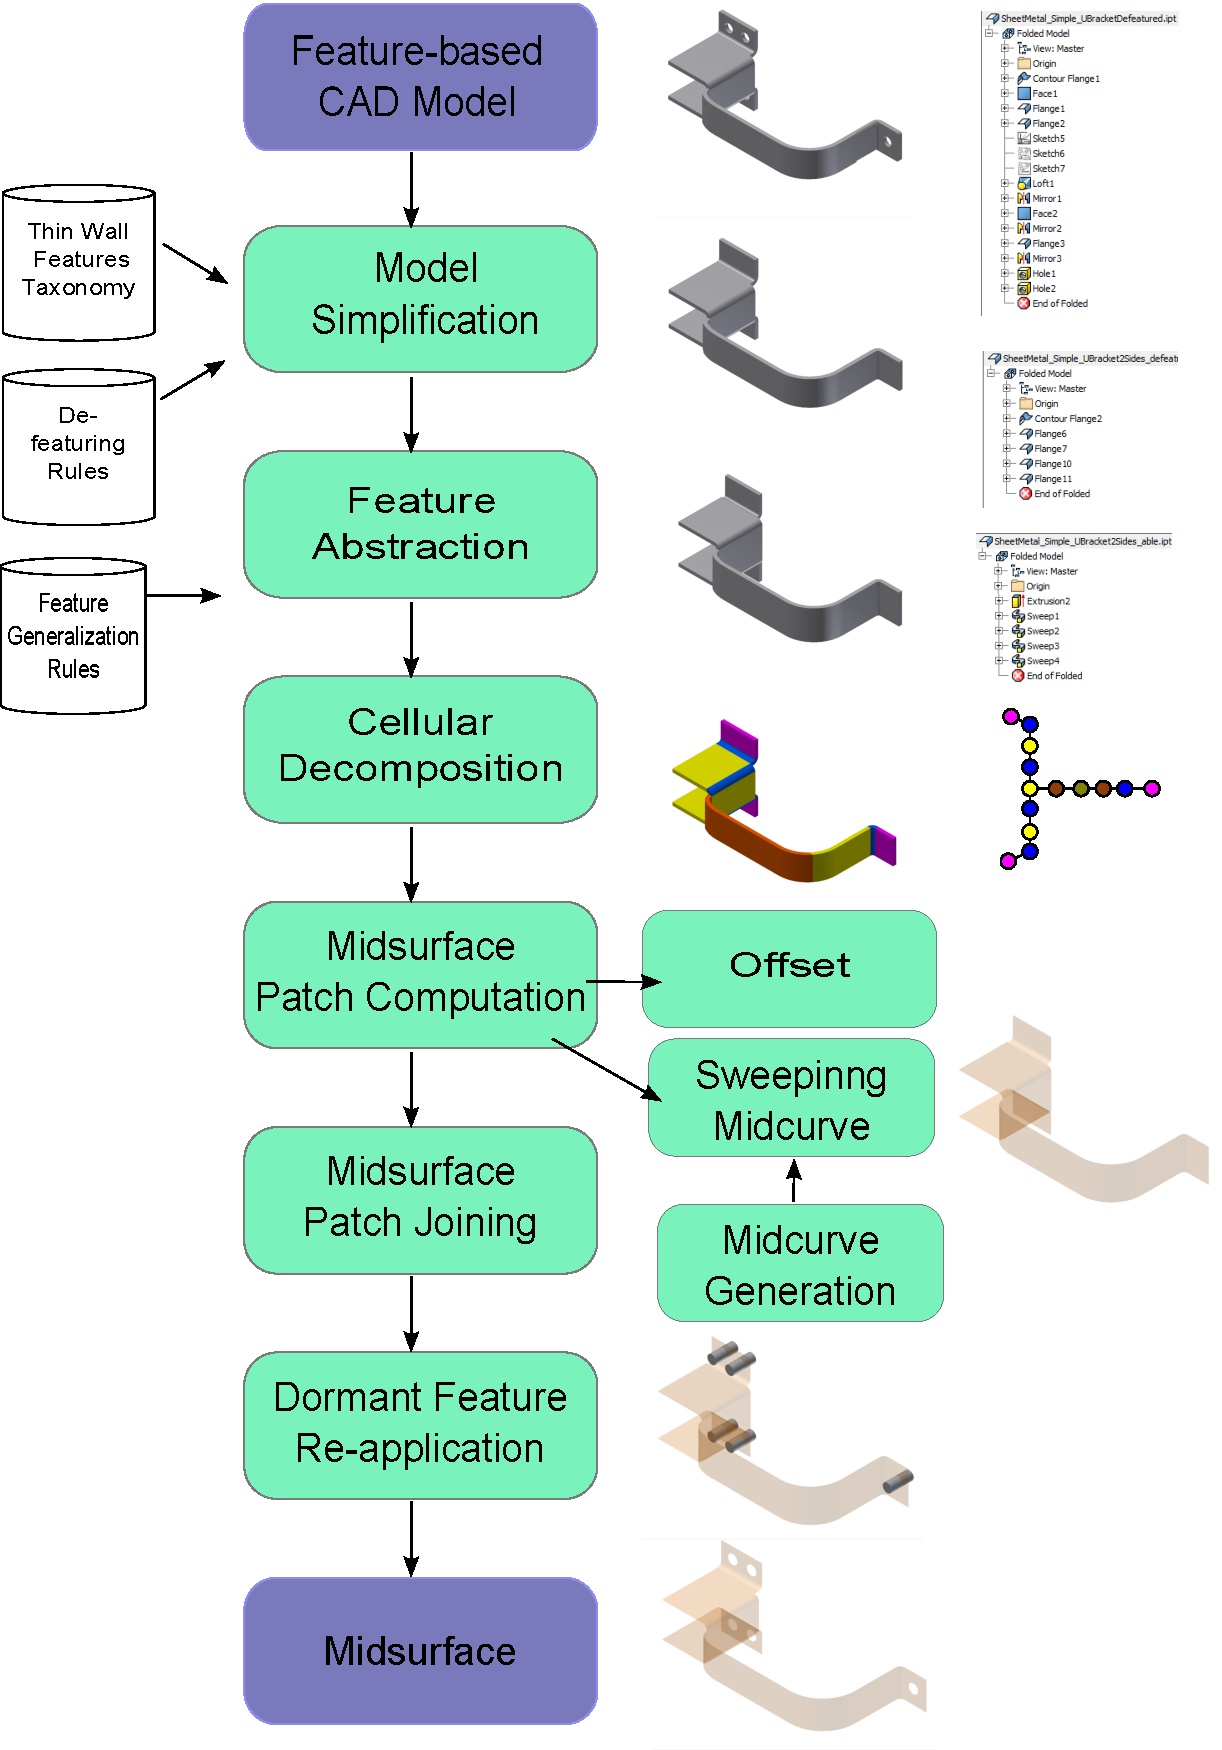
\includegraphics[width=0.5\linewidth]{../Common/images/SystemArchitecture_nolabels_5.pdf}
	\caption{Overall work-flow}
	\label{fig_sysarch}
    \end{figure}

\begin{itemize}[noitemsep,topsep=2pt,parsep=2pt,partopsep=2pt]
\item \textbf{Input}: Input to the system is sheet metal feature-based CAD model. 

\item \textbf{Model Simplification}: Features which do not impact the gross shape are removed. Out of remaining features, the negative features are removed after caching their tool bodies, to be used later for re-applying on the midsurface \cite{YogeshCADConf2015} (elaborated in section \ref{cagd:sec:defeaturing}). %\footnote{Terms ``Defeaturing'' and ``Simplification'' are used synonymously in this work unless specified otherwise}

\item \textbf{Feature Abstraction}: CAD features of the simplified model are transformed to generalized feature forms \cite{YogeshIITG2014}  (elaborated in  section  \ref{cagd:sec:abstraction}). %\footnote{Terms ``Generalization'' and ``Abstraction'' are used synonymously in this work unless specified otherwise}

\item \textbf{Model Decomposition}: Abstracted model is then decomposed into volumetrically-adjacent cellular bodies, each with a link to its respective owner feature. Cellular bodies are  classified into midsurface-patch generating cells (solid cells) and patch-joining cells (interface cells).

\item \textbf{Midsurface Patch Generation}: Solid cells generate their own midsurface patch by either of following methods:
\begin{itemize}[noitemsep,topsep=2pt,parsep=2pt,partopsep=2pt]
\item Offset: In case the profile is far bigger than the guide, profile face is offset-ed half way to get the midsurface patch.
\item Midcurve: In case the profile is far smaller than the guide, midcurve of the profile is generated (using the proposed \textbf{Midcurve Generation} technique, and it is then swept along the guide curve to get the midsurface.
\end{itemize}
\item \textbf{Midsurface Patch Joining}: Interface cells extend and join all the midsurface patches incident upon them.
\item \textbf{Dormant Re-application}: Once the connected midsurface is ready, cached dormant tool-bodies are applied/pierced to get the final midsurface.

\item \textbf{Validation}: A newly proposed topological methodology is used, along with the geometrical methods to assess the quality of the resultant midsurface \cite{YogeshCADandA2015} (elaborated more in section \ref{cagd:sec:validation}).

\item \textbf{Output}: Output of the system is a well-connected midsurface is then sent to downstream applications such as CAE.
\end{itemize}

%In comparison with the previous approaches, the proposed one  (Figure  \ref{fig_sysarch}) addresses problems (Section \ref{sec:litsurvey:analysis}), by effective leveraging feature information in defeaturing and abstraction, and thus removes the need of error-prone face-pairing or feature recognition. It utilizes feature-based-cellular decomposition to make connection logic generic by reducing it to type-independent rules. 
The following sections provide details of each of the above-mentioned modules. 
%This report presents aggregate work-flow of these modules which have been individually presented in the past publications \cite{YogeshCOEP2013,YogeshIITM2013, YogeshCADConf2015, YogeshIITG2014, YogeshETES2014, YogeshIJCAET2017, YogeshCADandA2015}.

\section{Model Simplification of Sheet Metal feature-based CAD Model} \label{cagd:sec:defeaturing}
The objective of this module is to remove features that do not impact the overall/primary/gross shape of the model. The selection of candidate features for removal is based on the newly proposed sheet metal feature taxonomy. The taxonomy presents a classification of sheet metal features aimed at suggesting relevance of features in the context of generating the ``gross shape''.

\subsection{Sheet Metal Features Taxonomy}\label{sec:defeaturing:taxonomy}

Taxonomy is represented by ``vocabulary'' and ``structure'' and in the context of the proposed research it is a scheme to represent and classify features for a particular purpose, i.e. of generating the gross shape.

\begin{minipage}[c]{0.8\linewidth}
\begin{minipage}[t]{0.5\linewidth}
\begin{itemize}
[noitemsep,topsep=2pt,parsep=2pt,partopsep=2pt]
\item \textbf{Primary Features}: These are not removed irrespective of their size as they form the principal/gross shape.  Their absence will create missing midsurface patches. Examples:
	\begin{itemize} [noitemsep,topsep=2pt,parsep=2pt,partopsep=2pt]
	\item Face-Wall
	\item Flange
	\item Drawing
	\end{itemize}
\item \textbf{Secondary Features}: These are removed based on their relative smaller size with respect to the overall input-model and the size-threshold.  
 Examples:
	\begin{itemize} [noitemsep,topsep=2pt,parsep=2pt,partopsep=2pt]
	\item Stamping
	\item Emboss 
	\end{itemize}
	
\item \textbf{Tertiary/Auxiliary Features}: They are helper/ancillary shapes and thus, not a part of the gross/overall shape. So they can be removed irrespective of their sizes.
Examples:
	\begin{itemize} [noitemsep,topsep=2pt,parsep=2pt,partopsep=2pt]
	\item Lip
	\item Rest 
	\end{itemize}
	
%\item \textbf{Connecting Features}: These are not suppressed irrespective of their sizes, as removing them, will create gaps between the sub-shapes of the original part. Lacking these would create gaps, so these are retained irrespective of their relative size, small or large.
%Example is:
%	\begin{itemize} [noitemsep,topsep=2pt,parsep=2pt,partopsep=2pt]
%	\item Bend
%	\end{itemize}
		
\item \textbf{Feature Groups}: These are feature collections. Their irrelevance is evaluated as a collection with the size-based criterion. 	Examples:
\begin{itemize} [noitemsep,topsep=2pt,parsep=2pt,partopsep=2pt]
	\item Mirror
	\item Patterns
	\end{itemize}
\end{itemize}

\end{minipage}
\hfill
\begin{minipage}[t]{0.48\linewidth}
\begin{minipage}[t]{\linewidth}
\dirtree{%
.1 Sheet Metal Features.
.2 Primary Features.
.3 Face-Wall   \adjustbox{valign=t}{
\includegraphics[scale=0.65]{..//Common/images/InventorWall.png}}.
.3 Flange  \quad \adjustbox{valign=t}{
\includegraphics[scale=0.65]{..//Common/images/InventorFlange.png}}.
.3 Bend   \qquad \adjustbox{valign=t}{
\includegraphics[scale=0.65]{..//Common/images/InventorBend.png}}.
%.3 Loft Flange  \qquad \adjustbox{valign=t}{
\includegraphics[scale=0.65]{..//Common/images/InventorLoftedFlange.png}}.
%.3 Rib \quad \quad  \adjustbox{valign=t}{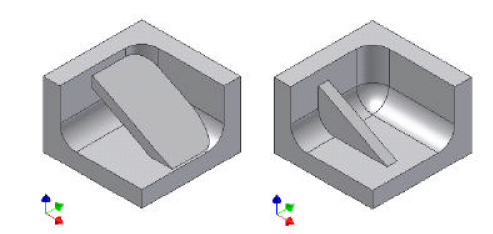
\includegraphics[height=0.11\linewidth]{..//Common/images/Feature_Rib.png}}.
.2 Secondary Features.
.3 Stamping  \quad \adjustbox{valign=t}{
\includegraphics[scale=0.65]{..//Common/images/InventorStamping.png}}.
.3 Cutout  \qquad \adjustbox{valign=t}{
\includegraphics[scale=0.65]{..//Common/images/InventorCutout.png}}.
%.3 Fold  \qquad \adjustbox{valign=t}{
\includegraphics[scale=0.65]{..//Common/images/InventorFold.png}}.
%.3 Roll  \qquad \adjustbox{valign=t}{
\includegraphics[scale=0.65]{..//Common/images/InventorRoll.png}}.
.3 Emboss \qquad \adjustbox{valign=t}{
\includegraphics[scale=0.65]{..//Common/images/InventorEmboss.png}}.
%.3 Hem   \quad \qquad \adjustbox{valign=t}{
\includegraphics[scale=0.65]{..//Common/images/InventorHem.png}}.
%.3 Grill \qquad \adjustbox{valign=t}{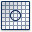
\includegraphics[scale=0.65]{..//Common/images/InventorGrill.png}}.
.2 Tertiary/Auxiliary Features.
%.3 Chamfer \qquad \adjustbox{valign=t}{
\includegraphics[scale=0.65]{..//Common/images/InventorChamfer.png}}.
%.3 Round  \qquad \adjustbox{valign=t}{
\includegraphics[scale=0.65]{..//Common/images/InventorRound.png}}.
%.3 Thread \qquad \adjustbox{valign=t}{
\includegraphics[scale=0.65]{..//Common/images/InventorThread.png}}.
.3 Lip \qquad \adjustbox{valign=t}{
\includegraphics[scale=0.65]{..//Common/images/InventorLip.png}}.
.3 Rest \qquad \adjustbox{valign=t}{
\includegraphics[scale=0.65]{..//Common/images/InventorRest.png}}.
%.2 Connecting Features.
%.3 Bend   \qquad \adjustbox{valign=t}{
\includegraphics[scale=0.65]{..//Common/images/InventorBend.png}}.
.2 Features Groups.
.3 Mirror \quad  \quad \adjustbox{valign=t}{
\includegraphics[scale=0.65]{..//Common/images/InventorMirror.png}}.
%.3 RectPattern \quad  \adjustbox{valign=t}{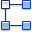
\includegraphics[scale=0.65]{..//Common/images/InventorRectPattern.png}}.
.3 Pattern\quad  \adjustbox{valign=t}{
\includegraphics[scale=0.65]{..//Common/images/InventorCircPattern.png}}.
}
\captionof{figure}{Proposed taxonomy (Icons source: \cite{Inventor2014Help})}\label{fig:tax_sm}
\end{minipage}

\begin{minipage}[t]{\linewidth}
\centering 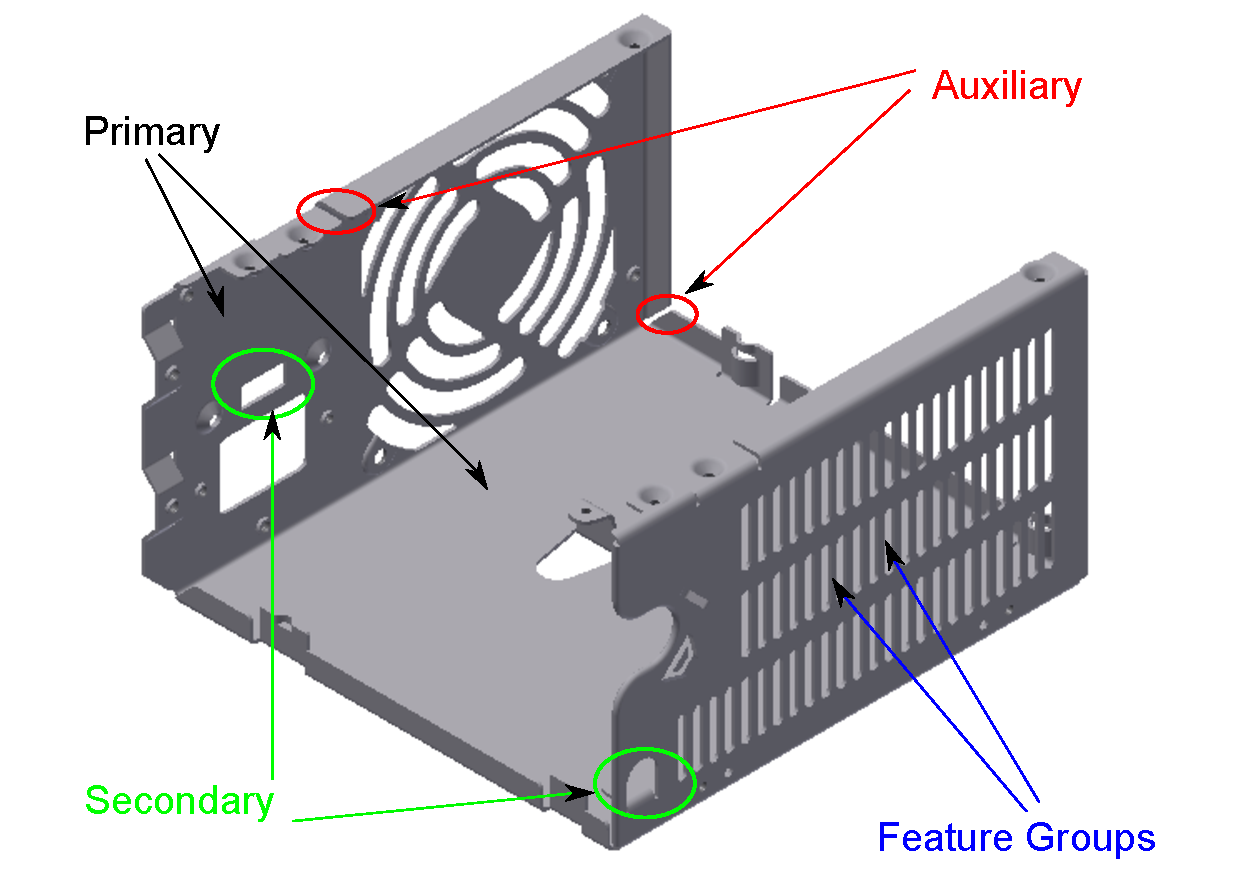
\includegraphics[width=0.8\linewidth]{..//Common/images/SheetMetal_taxonomy.pdf}
\captionof{figure}{Examples of classified types}\label{fig:classification}
\end{minipage}

\end{minipage}
\end{minipage}    

\bigskip

Model simplification is carried out in three phases as mentioned below.

\subsection{Phase I - Sheet Metal Features specific Model Simplification}\label{ph1}

A newly proposed taxonomy (Figure ~\ref{fig:tax_sm}) is used to decide the candidature of the sheet metal features for removal, as stated below:

%\smallskip

%%
%%%\subsubsection{Sheet Metal features taxonomy}
%%
%%\begin{figure}[!htb]
%%
%%\dirtree{%
%%.1 Sheet Metal Features.
%%.2 Primary Features.
%%.3 Face-Wall   \adjustbox{valign=t}{
\includegraphics[scale=0.65]{..//Common/images/InventorWall.png}}.
%%.3 Flange  \quad \adjustbox{valign=t}{
\includegraphics[scale=0.65]{..//Common/images/InventorFlange.png}}.
%%.3 Bend   \qquad \adjustbox{valign=t}{
\includegraphics[scale=0.65]{..//Common/images/InventorBend.png}}.
%%%.3 Loft Flange  \qquad \adjustbox{valign=t}{
\includegraphics[scale=0.65]{..//Common/images/InventorLoftedFlange.png}}.
%%%.3 Rib \quad \quad  \adjustbox{valign=t}{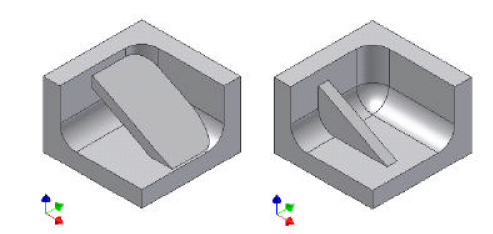
\includegraphics[height=0.11\linewidth]{..//Common/images/Feature_Rib.png}}.
%%.2 Secondary Features.
%%.3 Stamping  \quad \adjustbox{valign=t}{
\includegraphics[scale=0.65]{..//Common/images/InventorStamping.png}}.
%%.3 Cutout  \qquad \adjustbox{valign=t}{
\includegraphics[scale=0.65]{..//Common/images/InventorCutout.png}}.
%%%.3 Fold  \qquad \adjustbox{valign=t}{
\includegraphics[scale=0.65]{..//Common/images/InventorFold.png}}.
%%%.3 Roll  \qquad \adjustbox{valign=t}{
\includegraphics[scale=0.65]{..//Common/images/InventorRoll.png}}.
%%.3 Emboss \qquad \adjustbox{valign=t}{
\includegraphics[scale=0.65]{..//Common/images/InventorEmboss.png}}.
%%%.3 Hem   \quad \qquad \adjustbox{valign=t}{
\includegraphics[scale=0.65]{..//Common/images/InventorHem.png}}.
%%%.3 Grill \qquad \adjustbox{valign=t}{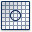
\includegraphics[scale=0.65]{..//Common/images/InventorGrill.png}}.
%%.2 Tertiary/Auxiliary Features.
%%%.3 Chamfer \qquad \adjustbox{valign=t}{
\includegraphics[scale=0.65]{..//Common/images/InventorChamfer.png}}.
%%%.3 Round  \qquad \adjustbox{valign=t}{
\includegraphics[scale=0.65]{..//Common/images/InventorRound.png}}.
%%%.3 Thread \qquad \adjustbox{valign=t}{
\includegraphics[scale=0.65]{..//Common/images/InventorThread.png}}.
%%.3 Lip \qquad \adjustbox{valign=t}{
\includegraphics[scale=0.65]{..//Common/images/InventorLip.png}}.
%%.3 Rest \qquad \adjustbox{valign=t}{
\includegraphics[scale=0.65]{..//Common/images/InventorRest.png}}.
%%%.2 Connecting Features.
%%%.3 Bend   \qquad \adjustbox{valign=t}{
\includegraphics[scale=0.65]{..//Common/images/InventorBend.png}}.
%%.2 Features Groups.
%%.3 Mirror \quad  \quad \adjustbox{valign=t}{
\includegraphics[scale=0.65]{..//Common/images/InventorMirror.png}}.
%%%.3 RectPattern \quad  \adjustbox{valign=t}{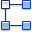
\includegraphics[scale=0.65]{..//Common/images/InventorRectPattern.png}}.
%%.3 Pattern\quad  \adjustbox{valign=t}{
\includegraphics[scale=0.65]{..//Common/images/InventorCircPattern.png}}.
%%}
%%
%%\caption{Sheet Metal features taxonomy (Icons source: \cite{Inventor2014Help})}\label{fig:tax_sm}
%%\end{figure}
%%
%%
%%
%%\begin{itemize}
%%[noitemsep,topsep=2pt,parsep=2pt,partopsep=2pt]
%%\item \textbf{Primary Features}: These are not suppressed irrespective of their size as they form the principal/gross shape.  Their absence will create missing midsurface patches. Examples:
%%	\begin{itemize} [noitemsep,topsep=2pt,parsep=2pt,partopsep=2pt]
%%	\item Face-Wall
%%	\item Flange
%%	\item Drawing
%%	\end{itemize}
%%\item \textbf{Secondary Features}: These are suppressed based on their relative smaller size with respect to the overall input-shape and the size-threshold. 
%% Examples:
%%	\begin{itemize} [noitemsep,topsep=2pt,parsep=2pt,partopsep=2pt]
%%	\item Stamping
%%	\item Emboss 
%%	\end{itemize}
%%	
%%\item \textbf{Tertiary/Auxiliary Features}: They are helper/ancillary shapes and thus, not a part of the gross/overall shape. So they can be suppressed irrespective of their sizes.
%%Examples:
%%	\begin{itemize} [noitemsep,topsep=2pt,parsep=2pt,partopsep=2pt]
%%	\item Lip
%%	\item Rest 
%%	\end{itemize}
%%	
%%\item \textbf{Feature Groups}: These are feature collections. Their suppressibility is evaluated as a collection with the size-based criterion. 	Examples:
%%\begin{itemize} [noitemsep,topsep=2pt,parsep=2pt,partopsep=2pt]
%%	\item Mirror
%%	\item Patterns
%%	\end{itemize}
%%\end{itemize}
%%
%%\begin{algorithm}[!h]
%%	\caption{Sheet metal Defeaturing}
%%	\label{alg:defeaturing:phase1}
%%	\begin{algorithmic}
%%		\REQUIRE A CAD model with access to the feature tree
%%		\WHILE{$nextFace() != null$}
%%			\STATE $F_i = currentFace()$
%%			\STATE $Area_{face} \quad += F_i \rightarrow area()$
%%		\ENDWHILE		
%%		\STATE $p = getInputFromUser()$
%%		\STATE $D = \frac{p}{100} \times Area$  \hspace{60mm}% //threshold size
%%		\WHILE{$nextFeature() != null$}
%%			\STATE $f_i = currentFeature()$
%%			\IF {$f_i \rightarrow isPrimaryFeature()$}
%%				\STATE continue
%%			\ELSIF {$f_i \rightarrow isTertiaryFeature()$}
%%				\STATE $sl \rightarrow add(f_i)$
%%			\ELSIF {$f_i \rightarrow isGroupFeature()$}
%%			  	\STATE $Area_{feature} = f_i \rightarrow combinedArea()$ \hspace{20mm}  %// Total area of the constituent features
%%			  	\IF {$Area_{feature}< D$}
%%			  		\STATE $sl \rightarrow add(f_i)$
%%				\ENDIF
%%			\ELSE      
%%				\STATE size $Area_{feature} = f_i \rightarrow area()$  // secondary feature
%%			  	\IF {$Area_{feature} < D$}
%%			  		\STATE $sl \rightarrow add(f_i)$
%%				\ENDIF				
%%			\ENDIF
%%		\ENDWHILE
%%		\STATE  $sl \rightarrow suppress()$
%%		%\STATE  $validate()$
%%	\end{algorithmic}
%%\end{algorithm}
%%
%%%\vspace{-1cm}



%\subsubsection{Phase I: Sheet Metal Taxonomy based Defeaturing Algorithm}
%The following steps identify the sheet metal features as per the classification presented in section \ref{ph1}. The identification uses the feature tree available as part of the feature based CAD model.
\begin{enumerate}
[noitemsep,topsep=2pt,parsep=2pt,partopsep=2pt]

%\item A List  ({\bf $sl$}) initialized to which the irrelevant features are added. 
\item The model feature tree is traversed and the candidate features for removal are identified based on a set of heuristic criteria such as ``Primary features are not to be removed'', ``Secondary features, if small, are selected'' etc.  (Figure \ref{fig:tax_sm}).
\item The identified features are added to the `candidates list'.
%\item The `candidates list' is presented to the user for verification and changes, if necessary. 
\item Features in the `candidates list' are removed.
%\item The model is regenerated and Defeaturing Effectiveness is computed using Eqn. \ref{eqn:defeaturing:effectiveness}
\end{enumerate}

Figure \ref{fig:phaseI} shows results of an example:

\begin{minipage}[t]{0.9\linewidth}
\begin{tabular}[h]{@{} p{0.3\linewidth} | p{0.3\linewidth} | p{0.3\linewidth}@{}} \toprule

\textbf{Input Model} & \textbf{Candidate Features} & \textbf{Simplified Output} \\ \midrule

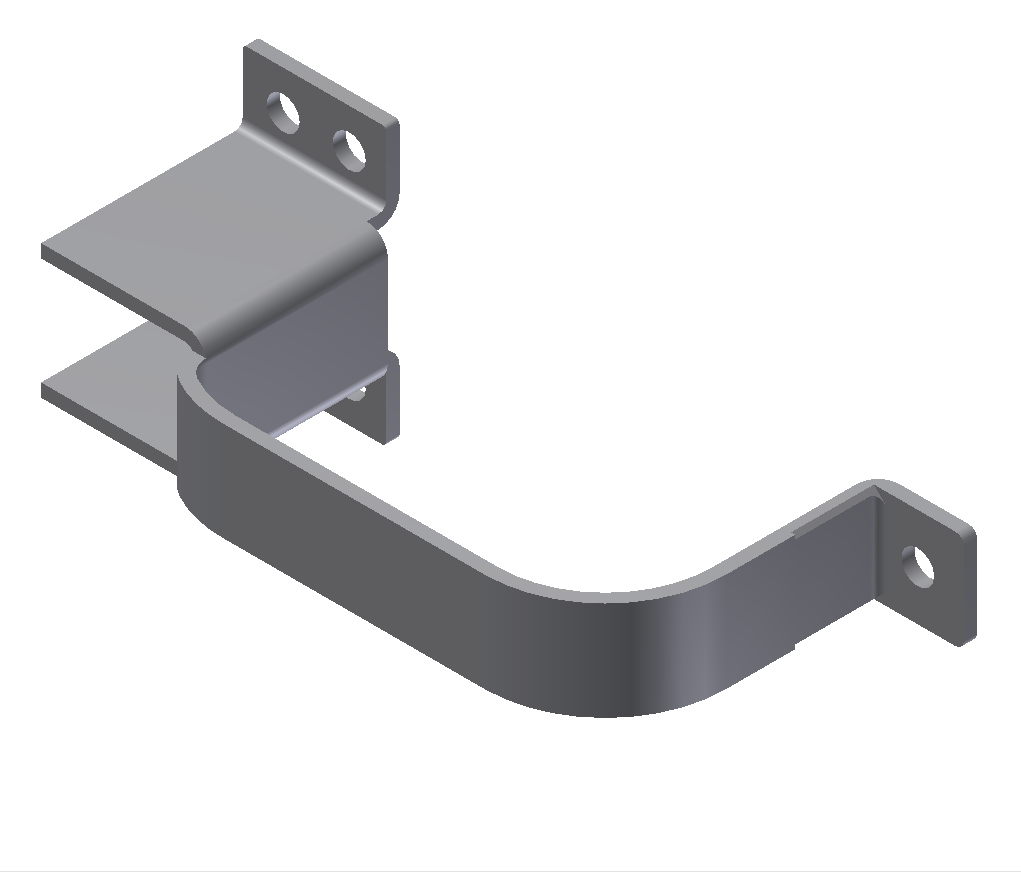
\includegraphics[width=0.98\linewidth]{..//Common/images/DefeatBracketPhase_I_1} &
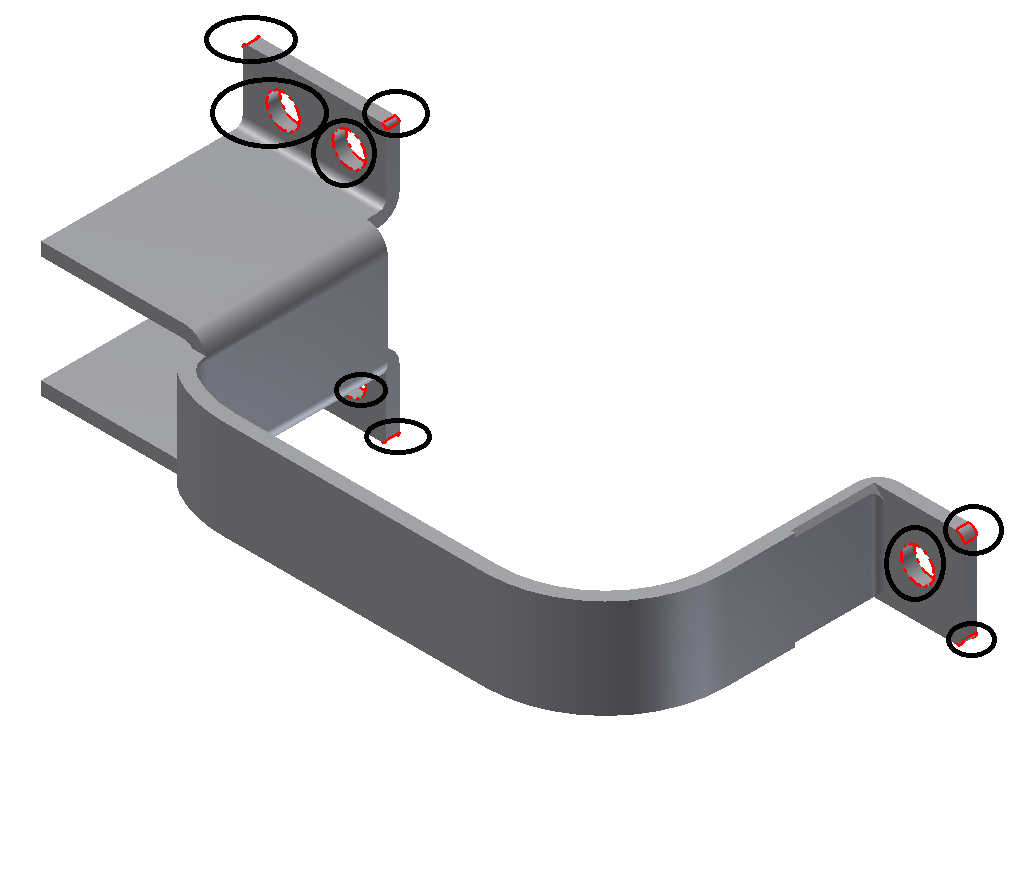
\includegraphics[width=0.98\linewidth]{..//Common/images/DefeatBracketPhase_I_2_circled} &
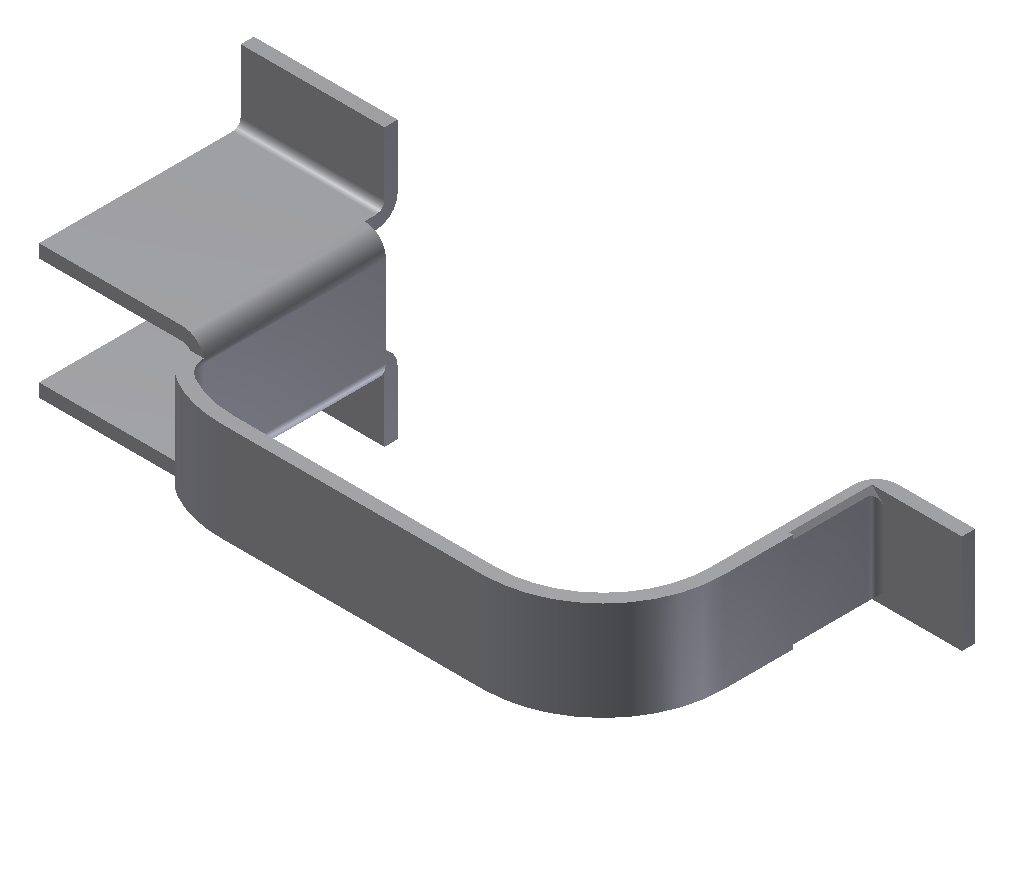
\includegraphics[width=0.98\linewidth]{..//Common/images/DefeatBracketPhase_I_3} \\ \bottomrule

\end{tabular}
\captionof{figure}{Phase I - Sheet Metal Features specific Model Simplification}\label{fig:phaseI}
\end{minipage}

\subsection{Phase II - Remnant Feature Volume based Model Simplification} \label{ph2}
CAD models are built using `design-by-features' approach. At each form-feature step, the feature parameters generate the ``tool-body'' portion first, which is booleaned to the model built till then. During this operation, some portion of the tool-body-portion gets consumed. Only the remaining (remnant) portion of the feature remains in the final model (Figure ~\ref{fig_remnant}). Identification of removable features based on the feature volume computed from the full feature parameters, thus, yields incorrect results \cite{Russ2012} as the final model may not retain the full feature volume. So, this work uses the size of remnant feature volume to decide the irrelevance (Figure ~\ref{fig_remnant}).

\begin{minipage}{0.9\textwidth}

\begin{minipage}[c]{0.33\linewidth}
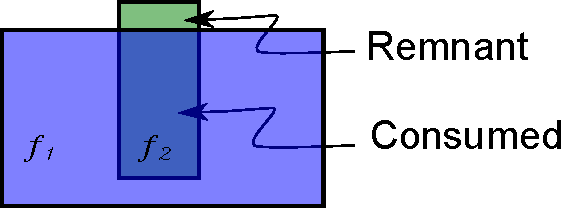
\includegraphics[width=\linewidth,valign=t]{../Common/images/Solid_Simple_SmallProtrusion.pdf}
\captionof{figure}{Remnant and Consumed portions of $f_2$} \label{fig_remnant}
\end{minipage}
\hfill
\begin{minipage}[c]{0.3\linewidth}
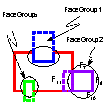
\includegraphics[width=0.8\linewidth,valign=t]{../Common/images/facegroups.pdf}
\captionof{figure}{Face Groups} \label{fig_clusters}
\end{minipage}
%%\begin{figure}[!h]%[!h]
%%\centering     
%%\subfloat[Remnant and Consumed portions of $f_2$]{\label{fig_remnant}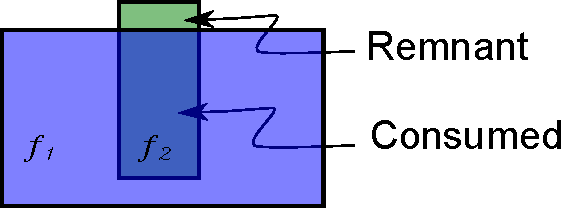
\includegraphics[width=0.5\linewidth,valign=t]{../Common/images/Solid_Simple_SmallProtrusion.pdf}} \quad
%%\subfloat[Formation of clusters]{\label{fig_clusters}\includegraphics[width=0.25\linewidth,valign=t]{../Common/images/clusters.pdf}}
%%\caption{Phase II: Remnant feature definition, Cluster approach} 
%%\label{fig:defeaturing:phaseII}
%%\end{figure}
\hfill
\begin{minipage}[c]{0.3\linewidth}
\begin{tabular}[h]{@{} p{0.4\linewidth} p{0.2\linewidth} p{0.3\linewidth}@{}} \toprule
\textbf{Face-groups} & \textbf{Size}& \textbf{Feature}\\ \midrule
FaceGroup$_1$ & 0.25 	&  Extrude$_2$\\
FaceGroup$_2$ & 0.25  & Extrude$_3$\\
FaceGroup$_3$ & 0.125 & Hole$_1$\\ \bottomrule
%$f_{10}, f_{12}, f_{15}, f_{14}$ 	& Cluster$_4$\\ \bottomrule
\end{tabular}
\captionof{table}{Face-groups with Respective Sizes}
\label{tbl_clusters}
\end{minipage}

\end{minipage}


%%\begin{figure}[!h]%[!h]
%%\centering     
%%\subfloat[Remnant and Consumed portions of $f_2$]{\label{fig_remnant}\includegraphics[width=0.5\linewidth,valign=t]{../Common/images/Solid_Simple_SmallProtrusion.pdf}} \quad
%%\subfloat[Formation of clusters]{\label{fig_clusters}\includegraphics[width=0.25\linewidth,valign=t]{../Common/images/clusters.pdf}}
%%\caption{Phase II: Remnant feature definition, Cluster approach} 
%%\label{fig:defeaturing:phaseII}
%%\end{figure}
%%
%%\begin{tabular}[h]{@{} p{0.3\linewidth} p{0.3\linewidth} p{0.3\linewidth}@{}} \toprule
%%\textbf{Clusters} & \textbf{Size}& \textbf{Feature}\\ \midrule
%%cluster$_1$ & 0.25 	&  Extrude$_2$\\
%%cluster$_2$ & 0.25  & Extrude$_3$\\
%%cluster$_3$ & 0.125 & Hole$_1$\\ \bottomrule
%%%$f_{10}, f_{12}, f_{15}, f_{14}$ 	& Cluster$_4$\\ \bottomrule
%%\captionof{table}{ Clusters Evaluation for Suppressibility}
%%\label{tbl_clusters}
%%\end{tabular}

Steps for identification of features for removal, based on the Remnant Feature Volume are:


\begin{enumerate}
[noitemsep,topsep=2pt,parsep=2pt,partopsep=2pt]

\item For each remnant face in the final body, the feature to which belongs (owner), is extracted.
\item  Face-groups are formed with same owning features as shown in Figure \ref{fig_clusters}, where the dotted portions show the consumed feature portions and the circles show the remnant portions. 
\item Size of the face-group can be calculated by various approaches like Influence Volume \cite{SangHunLee2005} or the union of bounding-boxes, etc. This work uses summation of the area of the remnant faces (Table \ref{tbl_clusters}) as the `Size' criterion. 
\item Each face-group-owning feature(s) is added to the `candidates list'  if the its size is below the threshold value.
%%\item The candidates list is presented to the user for verification and changes, if necessary. 
\item Features in candidates list are removed.
%%\item The model is regenerated and Defeaturing Effectiveness is computed using Eqn. \ref{eqn:defeaturing:effectiveness}
\end{enumerate}

%%\begin{algorithm}[!tbh]
%%	\caption{Remnant Faces method}
%%	\label{alg:defeaturing:phase2}
%%	\begin{algorithmic}
%%		\REQUIRE A CAD model with access to the feature tree. 
%%		\WHILE{$nextFace() != null$}  
%%			\STATE $F_i = currentFace()$
%%			\STATE $feat = F_i \rightarrow owingFeature()$
%%			\STATE $addedFlag = false$
%%			\WHILE {$nextCluster() != null$}
%%				\STATE $cl_j = currentCluster()$
%%				\IF {$cl_j \rightarrow owingFeature() == feat$}
%%					\STATE  $cl_j \rightarrow add(F_i)$
%%					\STATE $addedFlag = true$
%%				\ENDIF
%%			\ENDWHILE
%%			\IF {$addedFlag == false$}
%%				\STATE  $cl_n = newCluster()$
%%				\STATE  $cl_n \rightarrow owingFeature() = feat$
%%				\STATE  $cl_n \rightarrow add(f_i)$
%%			\ENDIF
%%		\ENDWHILE
%%		\WHILE {$nextCluster() != null$}
%%			\STATE $cl_k = currentCluster()$
%%			\STATE $size = cl_k \rightarrow calculateSize()$
%%			\IF {$size < D$} %\hspace{40mm} // Threshold D defined in Alg \ref{alg1}
%%				\STATE   $sl \rightarrow add(cl_k)$
%%			\ENDIF			
%%		\ENDWHILE
%%		\STATE  $sl \rightarrow suppress()$
%%		\STATE  $validate()$
%%	\end{algorithmic}
%%\end{algorithm}

Figure \ref{fig:phaseII} shows results of an example:

\begin{minipage}[t]{0.9\linewidth}
\begin{tabular}[h]{@{} p{0.3\linewidth}| p{0.3\linewidth}|  p{0.3\linewidth}@{}} \toprule

\textbf{Input Model} & \textbf{Candidate Features} & \textbf{Simplified Output} \\ \midrule


\includegraphics[width=0.98\linewidth]{..//Common/images/DefeatBracketPhase_I_3} &
\includegraphics[width=0.98\linewidth]{..//Common/images/DefeatBracketPhase_II_2_circled} &
\includegraphics[width=0.98\linewidth]{..//Common/images/DefeatBracketPhase_II_3} \\ \bottomrule

\end{tabular}
\captionof{figure}{Phase II - Remnant Feature Volume based Model Simplification}\label{fig:phaseII}
\end{minipage}
%%
%%In this work, the effectiveness of model simplification is computed by means of  percentage reduction ($pR$) in the number of the faces while keeping the overall shape intact (\%):
%%	\begin{equation}\label{eqn:defeaturing:effectiveness}  pR = (1 - \frac{rF}{nF}) \times 100\end{equation}
%%	Where, 
%%	\begin{enumerate}
%%	[noitemsep,topsep=2pt,parsep=2pt,partopsep=2pt]
%%	\item Total number of the faces in the original part ($nF$)
%%	\item Number of faces left after Phase II ($rF$)
%%	\end{enumerate}
%%
%%More Defeaturing percentage is effective only till the relevant features are not lost.

\subsection{Phase III - Identification of Dormant Features}\label{sec:dormant}

\begin{minipage}{0.95\textwidth}
\begin{minipage}[c]{0.42\linewidth}
\includegraphics[width=0.75\linewidth,valign=t]{../Common/images/dormant}
\captionof{figure}{Dormant Feature Tool-body} \label{fig_dormant}
\end{minipage}
\hfill
\begin{minipage}[c]{0.56\linewidth}
Negative features (like Holes, Cuts) which constituent the `gross shape', are still the candidates for removal in this phase. They are removed after saving their tool-body portions. These bodies are kept dormant to be used later for re-application on the midsurface. By this deferment of processing dormant features, generating midsurface patches gets simplified as these features are not present during their computation. But once the midsurface is ready, they are re-applied so that their presence in the midsurface is not lost  (Figure \ref{fig_dormant}).% (Refer example in Section \ref{sec:results:computation} for more details).
\end{minipage}

\end{minipage}

\section{Transformation of CAD features to Generalized Feature-form}  \label{cagd:sec:abstraction}
The diversity of features poses problems in the development of generic algorithms. Features like {\em Box}, {\em Pad}, {\em Protrusion}, {\em Extrude}, appear different due to nomenclature, but all could be representing the same model. A standardized representation has been proposed using Affine Transformation ($\mathcal{A}$),  Boolean ($\mathcal{B}$) and Loft ($\mathcal{L}$) and Entities($\mathcal{E}$).  This, together, is called as {\bf $\mathcal{ABLE}$}. The representation scheme proposed here is loosely based upon Interactive Configuration Exploration  (ICE) scheme developed by Moustapha \cite{Hoda2005}, for architectural designs. Although some the fundamental entities and syntax are borrowed from ICE, the rest has been enhanced it to suit the mechanical CAD application, such as this research (for more details, refer \cite{YogeshIITG2014}).  

\begin{figure}[!h]
\centering     %%% not \center
\subfloat[Generic Loft feature]{\label{fig:abstraction:loftschematics}\includegraphics[width=0.4\linewidth,valign=t]{../Common/images/LoftPreview.pdf}} \quad
\subfloat[Loft Equivalents]{\label{fig:abstraction:extruderevolvesweepasloft}\includegraphics[width=0.3\linewidth,valign=t]{../Common/images//LoftExtrudeRevSwp.pdf}}
\caption{Loft and its equivalents}
\label{fig_lofts}
\end{figure}


Loft is proposed to be the generalized feature form (Figure \ref{fig:abstraction:loftschematics})  capable of representing  most of the CAD features, including the sheet metal features. It constitutes multiple {\em profiles} and a guide {\em curve}.  Features like Extrude, Revolve and Sweep are specialized cases of Loft and are thus regarded as Loft-equivalents (Figure \ref{fig:abstraction:extruderevolvesweepasloft}).
%
%\begin{figure}[htbp]
%	\includegraphics[scale=0.35]{../Common/images//LoftExtrudeRevSwp.pdf} 
%\caption{Extrude, Revolve and Sweep in terms of Loft}
%\label{fig:abstraction:extruderevolvesweepasloft}
%\end{figure}
%
%\begin{figure}[htbp]
%%\begin{tabular}{  p{0.22\textwidth}  p{0.22\textwidth} }
%
%	\includegraphics[scale=0.35]{../Common/images//LoftPreview.pdf} 
%	%\includegraphics[scale=0.3]{../Common/images//LoftProfilesPath.pdf} \\
%
%%\end{tabular}
%\caption{Generic Loft feature}
%\label{fig:abstraction:loftschematics}
%\end{figure}

%Strictly, $\mathcal{L}$oft is a more generic case where the body is created between more than one sketch along the guide curve. Any arbitrary Free From surface is a network of u-v curves and can be imagined as a $\mathcal{L}$oft of multiple $u$ curves along multiple $v$ curves. In this work, at places, Sweep (which is a single sketch and a single guide curve) is used synonymously for the purpose of clarity.

In this module, input feature tree is converted into Loft-equivalents' {\bf $\mathcal{ABLE}$} tree (Figure \ref{fig:abel}) \cite{YogeshIITG2014}. This abstracted tree is then sent for Midsurface generation. 
%%Loft is a generic operator (Figure \ref{figure_Loft})  capable of generating most of the basic shapes. It joins {\em profiles} along a guide {\em curve} and represented as \loft{}{subtype}{3}{0, curve, 0 | C_{0,1,2}}{ (sketch )^{<1-n>}}.  {\em Continuity} options like $C_0$ for connectedness, $C_1$ for tangency and $C_2$ for curvature continuity. Output of the Loft can either be a $solid$ (where capping faces are added to close the shape) or a $surface$ (capping faces are not added) and accordingly, dimensionality $2|3$ can be specified \footnote{Sweep is a specialized case of Loft (with a single profile and a guide curve).}.
%%
%%\begin{figure}[!htp]
%%	\centering
%%	\includegraphics[width=0.45\linewidth]{../Common/images//LoftPreview.pdf} 
%%	\caption{Generic Loft feature}
%%	\label{figure_Loft}
%%\end{figure}
The algorithms for transforming sheet metal CAD features are are illustrated in Table \ref{tbl:abstraction:sheetmetalfeaturesable}.

\begin{table}[!h]
  \centering
  \resizebox{0.92\linewidth}{!}{ 
\begin{tabular}[htp]{@{}p{0.2\linewidth} | p{0.2\linewidth} | p{0.5\linewidth}@{}}
\toprule
 {\bf Figure } & {\bf Feature} & {\bf Loft Equivalents ($\mathcal{ABLE}$)} \\ \midrule

\raisebox{-.9\height}{\includegraphics[width=0.98\linewidth]{..//Common/images/abs_face}} &  {\bf Face, Wall, Base Flange}  & 
{\bf Extrude} is created by extracting sketch of the ``Wall'  feature and giving sheet metal thickness as the distance for extrusion.
\\ \midrule
  \raisebox{-.9\height}{\includegraphics[width=0.98\linewidth]{..//Common/images/abs_bend}} & {\bf Bend}   & 
  {\bf Sweep} is created by creating path using bend radius and a planar section as profile
%	\begin{algorithmic}
%		\REQUIRE Two Edges
%		\STATE  From first edge, gets it corresponding planar (not rounded) face and create a profile out of it.
%		\STATE  Using bend radius and starting points of both edges, create path profile, then create the sweep
%	\end{algorithmic}
\\ \midrule

 \raisebox{-.9\height}{\includegraphics[width=0.98\linewidth]{..//Common/images/abs_flange}}  & {\bf Flange}   &  
  {\bf Sweep} is created by creating path using bend radius, offset distance and a planar section as profile
%	\begin{algorithmic}
%		\REQUIRE Edge , offset, Bend radius
%		\STATE  Face on which edge was selected is consumed, so we have to rollback before this flange, cache face's geometry as a polyline3d lines, then roll forward.
%		\STATE  The cached geom is then used to create 2 sketches, one for profile and one for path
%	\end{algorithmic}
\\ \midrule


 \raisebox{-.9\height}{\includegraphics[width=0.98\linewidth]{..//Common/images/abs_cflange}} &
{\bf Contour Flange }   &  
  {\bf Sweep} is created by creating path using contour path and a planar section as profile	
%  	\begin{algorithmic} 
%		\REQUIRE Contour Path , distance
%		\STATE  While in rollback state, cache curves of contour path and distance
%		\STATE  Create a new sketch and copy curves in. Offset the curves and add capping lines to make closed profile
%		\STATE Extrude the profile
%	\end{algorithmic}
	
%	\begin{algorithmic}
%		\REQUIRE Edge
%		\STATE  While in rollback state,  cache face data similar to FLANGE
%		\STATE  Move the face inside and then prepare contour path, similar to FLANGE
%		\STATE  SWEEP the profile and path
%	\end{algorithmic}
\\ \midrule

 \raisebox{-.9\height}{\includegraphics[width=0.98\linewidth]{..//Common/images/abs_hem}} & 
 {\bf Hem}   &  
   {\bf Sweep} is created by creating path using hem parameters and a planar section as profile	
%	\begin{algorithmic}
%		\REQUIRE Edge , gap, Bend radius
%		\STATE  Face on which edge was selected is consumed, so we have to rollback before this, cache face's geometry as a polyline3d lines, then roll forward
%		\STATE  The cached geom is then used to create 2 sketches, one for profile and one for path
%	\end{algorithmic}
\\

\bottomrule
\end{tabular}
}
\caption{Loft equivalents ($\mathcal{ABLE}$) of Sheet Metal features}
\label{tbl:abstraction:sheetmetalfeaturesable}
\end{table}


Figure \ref{fig:abel} shows that the model remains the same only the features change. 
 
\begin{minipage}[t]{0.9\linewidth}
\begin{tabular}[h]{@{} p{0.24\linewidth} p{0.2\linewidth} |  p{0.24\linewidth}  p{0.2\linewidth}@{}} \toprule

\textbf{CAD Features} & \textbf{Model} & \textbf{$\mathcal{ABLE}$ Features} & \textbf{Model}\\ \midrule


\raisebox{-.9\height}{\includegraphics[width=0.98\linewidth]{..//Common/images/ABELBracketInputTree}}&
\raisebox{-.9\height}{\includegraphics[width=0.98\linewidth]{..//Common/images/ABELBracketInputPart}} &
\raisebox{-.9\height}{\includegraphics[width=0.98\linewidth]{..//Common/images/ABELBracketOutputTree}} &
\raisebox{-.9\height}{\includegraphics[width=0.98\linewidth]{..//Common/images/ABELBracketOutputPart}} \\ \bottomrule

\end{tabular}
\captionof{figure}{Transformation of Sheet Metal features to  Generalized/Abstracted ($\mathcal{ABLE}$) forms}\label{fig:abel}
\end{minipage}

\section{Generation of Midsurface from Simplified-Abstracted Model}  \label{sec:litsurvey:fbcdmidsurf}
After model-simplification and feature-abstraction, the $\mathcal{ABLE}$ feature tree is then decomposed by feature-based cellular decomposition (FbCD) in which the feature volumes are partitioned into cell-bodies in such a way that there is no volumetric overlap. However, the cells can touch others at the boundary faces (called ``cell-faces'') fully, but not partially (Figure \ref{fig_fbcd}). 
%\subsection{Feature-based Cellular Decomposition (FbCD)} \label{cagd:sec:decomposition}
Steps for partitioning abstracted CAD model into cells are:
\begin{itemize}[noitemsep,topsep=2pt,parsep=2pt,partopsep=2pt]
\item \textbf{Feature partitioning}: Internal as well as external booleans  are changed to the ``New Body'' type, so that the tool-body portions get separated.
\item \textbf{Concave edge partitioning (CEP)}: Overlapping tool-body portions are split at the concave edges, by extending adjacent faces.
\end{itemize}

FbCD leverages the CEP algorithm documented in the existing literature. Thus, as it is not the contribution of this work, is not elaborated in details.

%The $\mathcal{ABLE}$ feature tree is iterated and all the booleans (Internal/External) are changed to ``New Body'' type, so that the tool-body volumes are decoupled.
%Faces at concave edges are extended and used as partitions to split the volumes using already known approach such as Convex Partitioning. Extension does not happen indefinitely but within the influence zone decided by two interacting features.


\begin{figure}[!h]
\centering     %%% not \center
\subfloat[Original Part]{\label{fig_orig}\includegraphics[width=0.26\linewidth,valign=t]{../Common/images/DecompBracketInput}}
\subfloat[Decomposition]{\label{fig_cd}\includegraphics[width=0.25\linewidth,valign=t]{../Common/images/DecompBracketOutput}}
\subfloat[Before decomposition]{\label{fig_twofeat}\includegraphics[width=0.2\linewidth,valign=t]{../Common/images/FeatureInteractionMergedPart.pdf}} \quad
\subfloat[After decomposition]{\label{fig_featinteract}\includegraphics[width=0.2\linewidth,valign=t]{../Common/images//FeatureInteractionMergedCells.pdf}}
\caption{Examples of FbCD: Bracket Model and Schematic ``L'' shape}
\label{fig_fbcd}
\end{figure}

%Figure \ref{fig_twofeat} shows features $f_1$ and $f_2$ are interacting. Interaction can have full/partial volumetric/surface overlaps. 
%In the scenario shown above, volumes of $f_1$ and $f_2$ are partitioned in such a way that a common cell (with owner $f''_1f''_2$) is formed (Figure \ref{fig_featinteract}). Remaining portions of $f_1$ and $f_2$ are termed as $f'_1$ and $f'_2$ respectively.  Overlapping faces are denoted as $O_1$ and $O_2$. Thus, now, the cell-bodies do not overlap volumetrically [$O_{i,j}^3$], but may overlap at faces [$O_{i,j}^2$] fully [ $C_i \cap C_j = 0| O_{i,j}^2$].
%This FbCD technique scores over some of the past techniques such that partitioning does not populate too many/redundant cells due to global splitting  \cite{Chong2004, Kageura2009, Cao2011, Woo2009, Boussuge2013}. It also retains the feature ownerships, so that each cell knows the original Loft/Sweep feature to which it belongs and can query the corresponding profile and guide curve.
\subsection{Proposed Approach for Generation of Midsurface} \label{cagd:sec:compmids}
FbCD results in $n$ cell-bodies with owning-feature(s) assigned to each of them. A cell adjacency graph [CAG, $G(n,e)$] is formed with the $n$ nodes, each representing a cell-body. For each face-overlap between two nodes, an edge ($e$), having two nodes ($n$) attached on either end, is created in the CAG. Observing the connectivity at each cell-node, they are classified into solid cells ($sCell$) and interface cells ($iCell$). 
%Each node in CAG represents a feature sub-volume also known as cell-body. A cell body has three dimensions, the two sides of the aligned bounding box of the profile and the length of the guide curve (say, $d_1,d_2,d_3$). Nodes are classified as $sCell$s and $iCell$s as per the following definitions:
%\begin{mydef}
%\label{def:scell}
%Solid cell ($sCell$) is a cell-body where only one of its dimensions ($d_1$) is less than the threshold-factor ($t$) times any of the other two dimensions ($d_2, d_3$), denoted as  $d_1 < t.d_2 \quad \&  \quad d_1 < t.d_3$. 
%\end{mydef}
%\begin{mydef}
%\label{def:icell}
%Interface cell ($iCell$) is a cell-body where  both the minimum of the two dimensions ($d_1,d_2$)  are less than the threshold-factor ($t$) times of the maximum dimensions ($d_3$), denoted as  $d_1 < t.d_3 \quad \&  \quad d_2 < t.d_3$. 
%\end{mydef}
Fundamentally $sCell$s and $iCell$  are the building blocks of the model. Each contributes to the generation of midsurface by following rules:

\begin{myrule}
\label{rule:scell}
Solid cell ($sCell$) generates midsurface patch looking at its morphological characteristics of its owning Loft feature, basically relative sizes of the profile and the guide curve.
\end{myrule}
\begin{myrule}
\label{rule:icell}
Interface cell ($iCell$) connects all the midsurface patches incident upon it.
\end{myrule}

%Since generating a midsurface patch for $sCell$  is relatively straight-forward, these are discrete volumes with known owning-feature of only one type ``Loft''. For Loft (or for its equivalents like Sweep, Revolve, Extrude), the midsurface patch can be computed in a deterministic manner. The problem of resolving interaction amongst the midsurface patches is carried out in the $iCell$s, again in a reliable manner.
%
Advantage of the CAG representation is that it is easier to classify nodes based on cell characteristics and delegate specific computational work to each using generic rules. Thus, the proposed research does not need to enumerate specific heuristic rules used for specific connection types. Another advantage is that as the problem domain has been decomposed into manageable sub-problems, complexity of the original problem becomes irrelevant. Whatever the large/complex the original model may be, its constituent cells can be handled deterministically. Midsurface generation strategies for $sCell$s and  $iCell$s are detailed out in the sections below.
%			
\subsection{Generating of Midsurface Patches in Solid Cells}
\label{sec:scell}
A midsurface patch is generated looking at the feature parameters of owner Loft feature such as the profile $p$ and the guide curve $g$ \cite{YogeshIITG2014}.  For each Loft-equivalent feature, the midsurface patch can be generated in the following manner: 

\begin{itemize}[noitemsep,topsep=2pt,parsep=2pt,partopsep=2pt]

\item {\bf Midcurve}: If {\em profile} is very small compared to {\em curve} ( $profile_{length} \ll curve_{length}$), then {\em midcurve} (Section \ref{sec:midcurve}) is extracted from the {\em profile} and swept  along the guide {\em curve}.

\begin{figure}[h]
\centering \includegraphics[scale=0.5]{../Common/images//MidsurfSmallProfile_1.pdf} 
%\caption{sketch is far smaller than curve}
\label{figure_MidsurfSmallProfile}
\end{figure}

\vspace{-0.5cm}

\item {\bf Offset} :  If {\em profile} is very big as compared to {\em curve} ($profile_{length} \gg curve_{length}$), then {\em midcurve} is not extracted  but the {\em profile} itself is {\em swept} along half of the {\em curve}. 

\item {\bf Skip}:   If {\em sketch} is comparable in size to {\em curve}  ($sketch_{length} \approx curve_{length}$), then it is a thick shape and Midsurface is not generated.

\end{itemize}

%%Applying these strategies for $sCell$s shown in Figure \ref{fig_fbcd}, the corresponding midsurface-patches generated are shown in Figure \ref{fig_scells}. 
%%	
%%	
%%	\begin{figure}[!h]
%%	\centering     %%% not \center
%%	\subfloat[Patches, 2d view]{\label{fig_patches2d}\includegraphics[width=0.28\linewidth]{../Common/images/MidsurfPatches.pdf}} \qquad
%%	\subfloat[Patches, 3d view]{\label{fig_patches3d}\includegraphics[width=0.28\linewidth]{../Common/images/sCellMidsurfs3d}}
%%	\caption{Midsurface patches } 
%%	\label{fig_scells}
%%	\end{figure}
			
%%	\begin{algorithm}[!h]
%%		\caption{sCell midsurface patch computation}
%%		\label{alg_MidsurfsCell}
%%		\begin{algorithmic}
%%			\REQUIRE $sCell$
%%			\ENSURE $size(sCell \rightarrow owning-feature(s)) = 1$
%%			\STATE $f = sCell \rightarrow owning\_feature()$
%%			\STATE $p = f \rightarrow get\_profile()$
%%			\STATE $g = f \rightarrow get\_guide\_curve()$
%%			%\STATE $is\_thin\_profile = \sqrt{Area(profile)} < threshold \times length(guide)$ 
%%			\IF{$is\_thin\_profile(p) == true$}
%%				\STATE $m^1 = p\rightarrow compute\_midcurve()$
%%				\STATE $m^2 = sweep(m^1 ,g)$
%%			\ELSE
%%				\STATE $m^2 = offset(p ,g/2)$
%%			\ENDIF
%%		\end{algorithmic}
%%	\end{algorithm}
	
	

At this stage, the $sCell$s are filled with the midsurface patches and are ready to get connected in $iCell$s (section \ref{sec:icell}). Following section describes the proposed approach to generate midcurve.

\subsection{Generation of Midcurve} \label{sec:midcurve}
Midcurve is set of connected 2D curves lying midway of a 2D profile. This research focuses on 2D planar polygonal sketch profiles with an assumption that curved shapes can be converted to polygonal shape by faceting. In the first  phase of the generation, a  polygon is partitioned into primitive sub-polygons and then in the second phase, midcurve-segments are generated in the non-interface-polygons.  At the end, the individual midcurve-segments  are extended-joined to form a continuous set of curves mimicking the parent shape. 



%\vspace{-2.1cm}

\subsubsection{Polygon Decomposition}
A polygon can be partitioned into convex regions by eliminating all reflex (concave) vertices. This research enhances method by  Bayazit\cite{Bayazit} (more details in \cite{YogeshETES2014} \cite{YogeshIJCAET2017}).


\def\partitioncomparisionraise{0.08}
\def\partitioncomparisionfig{0.98}

\begin{table}[!h]
\resizebox{0.7\linewidth}{!}{
\begin{tabular}[h]{@{} p{0.31\linewidth} p{0.31\linewidth} p{0.31\linewidth}@{}}
\toprule



{\bf Profile } & {\bf Bayazit\cite{Bayazit}} & {\bf Proposed}\\
\midrule
%------------------------------------------------------------------------------------------------------------------------------------
%T &
\raisebox{\partitioncomparisionraise\height}{\includegraphics[width=\partitioncomparisionfig\linewidth]{..//Common/images/Ts.png}} &
\raisebox{\partitioncomparisionraise\height}{\includegraphics[width=\partitioncomparisionfig\linewidth]{..//Common/images/Tb.png}}&
\raisebox{\partitioncomparisionraise\height}{\includegraphics[width=\partitioncomparisionfig\linewidth]{..//Common/images/Tp.png}} \\


%------------------------------------------------------------------------------------------------------------------------------------
%Plus  &
\raisebox{\partitioncomparisionraise\height}{\includegraphics[width=\partitioncomparisionfig\linewidth]{..//Common/images/Pluss.png}} &
\raisebox{\partitioncomparisionraise\height}{\includegraphics[width=\partitioncomparisionfig\linewidth]{..//Common/images/Plusb.png}}&
\raisebox{\partitioncomparisionraise\height}{\includegraphics[width=\partitioncomparisionfig\linewidth]{..//Common/images/Plusp.png}} \\

%------------------------------------------------------------------------------------------------------------------------------------
%DoubleK  &
\raisebox{\partitioncomparisionraise\height}{\includegraphics[width=\partitioncomparisionfig\linewidth]{..//Common/images/DoubleKs.png}} &
\raisebox{\partitioncomparisionraise\height}{\includegraphics[width=\partitioncomparisionfig\linewidth]{..//Common/images/DoubleKb.png}}&
\raisebox{\partitioncomparisionraise\height}{\includegraphics[width=\partitioncomparisionfig\linewidth]{..//Common/images/DoubleKp.png}} \\

\bottomrule
\end{tabular}
}
\caption{Improvement over current partitioning algorithm}
\label{tbl:midcurves:partitioncomparision}
\end{table}

The resulting sub-polygons are sent for creating connected midcurves. 

\subsubsection{Midcurve Generation}

Decomposition gets the sub-polygons which are of primitive shapes making it easier to compute midcurves compared to original-input-whole shape.  Each decomposed sub-polygon creates its own midcurves based on the number of sides and aspect ratio. Following are the steps (Table \ref{tbl:midcurves:midcurvecomp}) for generating connected midcurve:

\bigskip

\begin{table}[!h]
\def \mytablemidcurvewidth{0.6}


\begin{tabular}[h]{@{}p{0.28\linewidth} | p{0.28\linewidth}| p{0.28\linewidth}@{}}  \toprule
Each partitioning edge inserted during the decomposition is called as a `chord'. &
Midcurves are generated for individual polygons that are longer length-wise on both sides of the `chord'. &
When curves do not meet at the chord', they are extended upto the midcurve. \\

\raisebox{-.9\height}{\includegraphics[width=\mytablemidcurvewidth\linewidth]{..//Common/images/midcurve_polydecomp.pdf}} &
\raisebox{-.9\height}{\includegraphics[width=\mytablemidcurvewidth\linewidth]{..//Common/images/midcurve_polymid.pdf}}  &
\raisebox{-.9\height}{\includegraphics[width=\mytablemidcurvewidth\linewidth]{..//Common/images/midcurve_extend.pdf}} 
\\ \bottomrule
\end{tabular} 
\caption{Steps for Generating Connected Midcurve}
\label{tbl:midcurves:midcurvecomp}
\end{table}

\bigskip

Following are the sample-profiles taken from past research papers, and along with the midcuves generated from the above-mentioned process.

\bigskip

\resizebox{0.9\linewidth}{!}{
\begin{tabular}[h]{@{}p{0.3\linewidth} | p{0.3\linewidth}| p{0.33\linewidth}@{}} \toprule

Glass profile by Fischer \cite{Elber1999}. &
Profile by Ramanathan \cite{Ramanathan2004}. &
Plastic Part profile by Sheen \cite{Sheen2010}. \\ \midrule
\raisebox{-.9\height}{\includegraphics[angle=90, width=\linewidth]{..//Common/images/Glassmc.png}} &
\raisebox{-.9\height}{\includegraphics[width=\linewidth]{..//Common/images/DoubleKmc.png}}  &
\raisebox{-.9\height}{\includegraphics[width=\linewidth]{..//Common/images/Sheen1mc.png}} 
\\ \bottomrule
\end{tabular} 
}


\subsection{Connecting Midsurface Patches in Interface Cells}
\label{sec:icell}
Input to this module is a CAG with midsurface patches generated at all the $sCell$s. The sole responsibility of $iCell$s is to connect the midsurface patches incident on them, either by extending the midsurface-patches from the adjacent $sCell$s or by generating new ones.  The CAG is used to traverse $iCell$s one by one. Each $iCell$ is connected with adjacent cells via edges $e$(s).  Each incident $e$ has two nodes, where one is the ``self'', i.e. the current $iCell$ and the second one is called the ``adjacent node''.  The ``adjacent node'' could be either a $sCell$ or an $iCell$.   For each $iCell$, the midsurface patch interactions are resolved using following rules:

\begin{myrule}
\label{def:sicell}
If the ``adjacent node'' is a $sCell$, the adjacent midsurface-patch is extended up to $iCell$'s centroid (Figure  \ref{fig_sextensions}). An intersection curve ($m^1$) is generated between the overlapping face ($O_{1,2}$) and the midsurface ($m^2$). This curve acts as a midcurve for the extension into the $iCell$. In case, where all the three cells are geometrically flat and relatively big, all are marked as  $sCell$s (not $iCell$s) and have no extensions (Figure \ref{fig_sextensions}).
\end{myrule}

\begin{myrule}
\label{def:iicell}
If the ``adjacent node'' is an $iCell(n_3)$, then an extra patch is created between the centroids of the two $iCell$s (Figure  \ref{fig_iextensions}). Thus, all the $iCell$s join the midsurface patches (Figure \ref{fig_icells}) to form a well-connected midsurface (Figure \ref{fig_iextensions}).
\end{myrule}

	\begin{figure}[!h]
	\centering     %%% not \center
	\subfloat[Adjustments]{\label{fig_icells}\includegraphics[width=0.28\linewidth,valign=t]{../Common/images/MidsurfJoining.pdf}}
	\subfloat[$sCell-iCell$]{\label{fig_sextensions}\includegraphics[width=0.28\linewidth,valign=t]{../Common/images/sCellExtension.pdf}}
	\subfloat[$iCell-iCell$]{\label{fig_iextensions}\includegraphics[width=0.28\linewidth,valign=t]{../Common/images/iCellExtension.pdf}}	
	\caption{Resolving Interactions in the $iCell$}
	\label{fig_resolveiCell}
	\end{figure}

%%	\begin{algorithm}[!h]
%%		\caption{$iCell$ midsurface patch interaction resolution}
%%		\label{alg_MidsurfiCell}
%%		\begin{algorithmic}
%%			\REQUIRE $iCell$
%%			\WHILE{$size(iCell \rightarrow edges) > 0$}
%%				\STATE $e_i = iCell \rightarrow edge$
%%				\STATE $n_s = iCell $	
%%				\STATE $n_o = e_i \rightarrow get\_adjacent\_node(n_s) $			
%%				\IF{$n_o \rightarrow type == sCell$}
%%					\STATE $m_o = n_o \rightarrow query\_midsurface()$
%%					\STATE $O_f = e_i \rightarrow overlapping\_face()$
%%					\STATE $m^1 = surf\_surf\_intersection(O_f, m_o)$
%%					\STATE $m^2 = extrude(m^1, n_o \rightarrow centroid)$
%%				\ELSIF{$n_o \rightarrow type == iCell$}
%%					\STATE $c^1_1= get\_curve\_at\_centroid(n_s)$
%%					\STATE $c^1_2 = get\_curve\_at\_centroid(n_o)$
%%					\STATE $m^2 = create\_patch(c^1_1, c^1_2)$
%%					\ENDIF
%%			\ENDWHILE
%%		\end{algorithmic}
%%	\end{algorithm}
%%	
	
%%	\begin{figure}[!h]
%%	\centering   
%%	\subfloat[Before Resolving]{\label{fig_overlapscell}\includegraphics[width=0.28\linewidth]{../Common/images/sCellMidsurfs3dOverlap_zoom}}\quad
%%	\subfloat[After Resolving]{\label{fig_overlapicell}\includegraphics[width=0.28\linewidth]{../Common/images/iCellMidsurfs3dOverlap_zoom}}
%%	\caption{$iCell$ resolving in  Overlap case} 
%%	\label{fig_icellsovrelap}
%%	\end{figure}

Following are various academic cases along with their midsurface outputs:
\begin{itemize}[noitemsep,topsep=2pt,parsep=2pt,partopsep=2pt]

\item {\bf L} : Two midsurface patches from $sCell$s joining in an edge in the blue $iCell$.  (Figure \ref{fig_L})
	\begin{figure}[!h]
	\centering     %%% not \center
	\subfloat[Model]{\label{fig_Lmodel}\includegraphics[width=0.22\linewidth]{../Common/images/nonCellularL}} \quad
	\subfloat[Decomposition]{\label{fig_Ldecomp}\includegraphics[width=0.22\linewidth]{../Common/images/CellularL}}
	\subfloat[2 $sCell$s, 1 $iCell$]{\label{fig_Lgraph}\includegraphics[width=0.22\linewidth]{../Common/images/L_cellsJoining.pdf}} \quad
	\subfloat[Midsurface]{\label{fig_Lmidsurf}\includegraphics[width=0.22\linewidth]{../Common/images/midsCellularL}}
	\caption{Midsurface for L Model} 
	\label{fig_L}
	\end{figure}
	
	\item {\bf T} : Three midsurface patches from $sCell$s joining in an edge in the $iCell$.  (Figure \ref{fig_T})
	\begin{figure}[!h]
	\centering     %%% not \center
	\subfloat[Model]{\label{fig_Tmodel}\includegraphics[width=0.22\linewidth]{../Common/images/nonCellularT}} \quad
	\subfloat[Decomposition]{\label{fig_Tdecomp}\includegraphics[width=0.22\linewidth]{../Common/images/CellularT}}
	\subfloat[3 $sCell$s, 1 $iCell$]{\label{fig_Tgraph}\includegraphics[width=0.22\linewidth]{../Common/images/T_cellsJoining.pdf}} \quad
	\subfloat[Midsurface]{\label{fig_Tmidsurf}\includegraphics[width=0.22\linewidth]{../Common/images/midsCellularT}}
	\caption{Midsurface for T Model } 
	\label{fig_T}
	\end{figure}
	
	\item {\bf Curved Y} : Topologically similar to {\bf T}, but differs in $sCell$ generations.  (Figure \ref{fig_CurvedY})
	\begin{figure}[!h]
	\centering     %%% not \center
	\subfloat[Model]{\label{fig_CurvedYmodel}\includegraphics[width=0.22\linewidth]{../Common/images/nonCellularCurvedY}} \quad
	\subfloat[Decomposition]{\label{fig_CurvedYdecomp}\includegraphics[width=0.22\linewidth]{../Common/images/CellularCurvedY}}
	\subfloat[3 $sCell$s, 1 $iCell$]{\label{fig_CurvedYgraph}\includegraphics[width=0.22\linewidth]{../Common/images/CurvedY_cellsJoining.pdf}} \quad
	\subfloat[Midsurface]{\label{fig_CurvedYmidsurf}\includegraphics[width=0.22\linewidth]{../Common/images/midsCellularCurvedY}}
	\caption{Midsurface for Curved Y Model } 
	\label{fig_CurvedY}
	\end{figure}	
	
	\item {\bf Wavy Tri} : Topologically similar to {\bf T}, but differs in $sCell$. $iCell$ is 3 sided.  (Figure \ref{fig_Wavy})
	\begin{figure}[!h]
	\centering     %%% not \center
	\subfloat[Model]{\label{fig_WavyYmodel}\includegraphics[width=0.22\linewidth]{../Common/images/nonCellularCurvedTri}} \quad
	\subfloat[Decomposition]{\label{fig_WavyYdecomp}\includegraphics[width=0.22\linewidth]{../Common/images/CellularCurvedTri}}
	\subfloat[3 $sCell$s, 1 $iCell$]{\label{fig_Wavygraph}\includegraphics[width=0.22\linewidth]{../Common/images/Wavy_cellsJoining.pdf}} \quad
	\subfloat[Midsurface]{\label{fig_CurvedYmidsurf}\includegraphics[width=0.22\linewidth]{../Common/images/midsCellularCurvedTri}}
	\caption{Midsurface for Wavy Model } 
	\label{fig_Wavy}
	\end{figure}		
	
	\item {\bf Plus} : Four midsurface patches from $sCell$s joining in an edge in the $iCell$.  (Figure \ref{fig_Plus})
	\begin{figure}[!h]
	\centering     %%% not \center
	\subfloat[Model]{\label{fig_Plusmodel}\includegraphics[width=0.22\linewidth]{../Common/images/nonCellularPlus}} \quad
	\subfloat[Decomposition]{\label{fig_Plusdecomp}\includegraphics[width=0.22\linewidth]{../Common/images/CellularPlus}}
	\subfloat[4 $sCell$s, 1 $iCell$]{\label{fig_Plusgraph}\includegraphics[width=0.22\linewidth]{../Common/images/Plus_cellsJoining.pdf}} \quad
	\subfloat[Midsurface]{\label{fig_Plusmidsurf}\includegraphics[width=0.22\linewidth]{../Common/images/midsCellularPlus}}
	\caption{Midsurface for Plus Model} 
	\label{fig_Plus}
	\end{figure}			
	
	\item {\bf Drafted Plus} : Topologically similar to {\bf Plus} but has drafted $sCell$s. (Figure \ref{fig_DraftedPlus})
	\begin{figure}[!h]
	\centering     %%% not \center
	\subfloat[Model]{\label{fig_DraftedPlusmodel}\includegraphics[width=0.22\linewidth]{../Common/images/nonCellularDraftPlus}} \quad
	\subfloat[Decomposition]{\label{fig_DraftedPlusdecomp}\includegraphics[width=0.22\linewidth]{../Common/images/CellularDraftPlus}}
	\subfloat[4 $sCell$s, 1 $iCell$]{\label{fig_DraftedPlusgraph}\includegraphics[width=0.22\linewidth]{../Common/images/DraftedPlus_cellsJoining.pdf}} \quad
	\subfloat[Midsurface]{\label{fig_DraftedPlusmidsurf}\includegraphics[width=0.22\linewidth]{../Common/images/midsCellularDraftPlus}}
	\caption{Midsurface for DraftedPlus Model} 
	\label{fig_DraftedPlus}
	\end{figure}		
	
	\item {\bf Overlap} : $iCell-iCell$ interaction. (Figure \ref{fig_Overlap})
	\begin{figure}[!h]
	\centering     %%% not \center
	\subfloat[Model]{\label{fig_Overlapmodel}\includegraphics[width=0.22\linewidth]{../Common/images/nonCellularOverlap}} \quad
	\subfloat[Decomposition]{\label{fig_Overlapdecomp}\includegraphics[width=0.22\linewidth]{../Common/images/CellularOverlap}}
	\subfloat[2 $sCell$s, 2 $iCell$s]{\label{fig_Overlapgraph}\includegraphics[width=0.22\linewidth]{../Common/images/Overlap_cellsJoining.pdf}} \quad
	\subfloat[Midsurface]{\label{fig_Overlapmidsurf}\includegraphics[width=0.22\linewidth]{../Common/images/midsCellularOverlap}}
	\caption{Midsurface for Overlap Model} 
	\label{fig_Overlap}
	\end{figure}					
	
	\item {\bf LPlus}  \cite{Woo2013} : $iCell-iCell$ and $sCell-iCll$ interactions. (Figure \ref{fig_LPlus})
	\begin{figure}[!h]
	\centering     %%% not \center
	\subfloat[Model]{\label{fig_LPlusmodel}\includegraphics[width=0.22\linewidth]{../Common/images/nonCellularZU}} \quad
	\subfloat[Decomposition]{\label{fig_LPlusdecomp}\includegraphics[width=0.22\linewidth]{../Common/images/CellularZU}}
	\subfloat[5 $sCell$s, 2 $iCell$s]{\label{fig_ZUgraph}\includegraphics[width=0.22\linewidth]{../Common/images/ZU_cellsJoining.pdf}} \quad
	\subfloat[Midsurface]{\label{fig_LPlusmidsurf}\includegraphics[width=0.22\linewidth]{../Common/images/midsCellularZU}}
	\caption{Midsurface for LPlus Model} 
	\label{fig_LPlus}
	\end{figure}					
\end{itemize}

%%
%%\newcommand \myColWidthFactora {0.22}
%%\begin{center}
%%\resizebox{0.75\linewidth}{!}{
%%\begin{tabular}[!htb]{@{}p{0.12\linewidth} p{\myColWidthFactora\linewidth} p{\myColWidthFactora\linewidth}  p{\myColWidthFactora\linewidth}  p{\myColWidthFactora\linewidth} @{}} \toprule
%%{\bf Name} & {\bf Part} &  {\bf Cellular}  & {\bf Graph} & {\bf Result} \\ \midrule  
%%
%%L & 
%%\adjustbox{valign=t}{\includegraphics[width=\linewidth]{../Common/images/nonCellularL}}  &  
%%\adjustbox{valign=t}{\includegraphics[width=\linewidth]{../Common/images/CellularL}}  &
%%\adjustbox{valign=t}{\includegraphics[width=\linewidth]{../Common/images/CellGraphL.pdf}} &  
%%\adjustbox{valign=t}{\includegraphics[width=\linewidth]{../Common/images/midsCellularL}} 
%%\\ \midrule
%%
%%T & 
%%\adjustbox{valign=t}{\includegraphics[width=\linewidth]{../Common/images/nonCellularT}}  &  
%%\adjustbox{valign=t}{\includegraphics[width=\linewidth]{../Common/images/CellularT}}  &
%%\adjustbox{valign=t}{\includegraphics[width=\linewidth]{../Common/images/CellGraphT.pdf}} &  
%%\adjustbox{valign=t}{\includegraphics[width=\linewidth]{../Common/images/midsCellularT}} 
%%\\ \midrule
%%
%%Curved Y & 
%%\adjustbox{valign=t}{\includegraphics[width=\linewidth]{../Common/images/nonCellularCurvedY}}  &  
%%\adjustbox{valign=t}{\includegraphics[width=\linewidth]{../Common/images/CellularCurvedY}}  &
%%\adjustbox{valign=t}{\includegraphics[width=\linewidth]{../Common/images/CellGraphY.pdf}} &  
%%\adjustbox{valign=t}{\includegraphics[width=\linewidth]{../Common/images/midsCellularCurvedY}} 
%%\\ \midrule
%%
%%Wavy Tri & 
%%\adjustbox{valign=c}{\includegraphics[width=0.8\linewidth]{../Common/images/nonCellularCurvedTri}}  &  
%%\adjustbox{valign=c}{\includegraphics[width=\linewidth]{../Common/images/CellularCurvedTri}}  &
%%\adjustbox{valign=c}{\includegraphics[width=0.8\linewidth]{../Common/images/CellGraphTri.pdf}} &  
%%\adjustbox{valign=c}{\includegraphics[width=\linewidth]{../Common/images/midsCellularCurvedTri}} 
%%\\ \midrule
%%
%%
%%Plus & 
%%\adjustbox{valign=t}{\includegraphics[width=\linewidth]{../Common/images/nonCellularPlus}}  &  
%%\adjustbox{valign=t}{\includegraphics[width=\linewidth]{../Common/images/CellularPlus}}  &
%%\adjustbox{valign=t}{\includegraphics[width=\linewidth]{../Common/images/CellGraphPlus.pdf}} &  
%%\adjustbox{valign=t}{\includegraphics[width=\linewidth]{../Common/images/midsCellularPlus}} 
%%\\ \midrule
%%
%%
%%Drafted Plus & 
%%\adjustbox{valign=t}{\includegraphics[width=\linewidth]{../Common/images/nonCellularDraftPlus}}  &  
%%\adjustbox{valign=t}{\includegraphics[width=\linewidth]{../Common/images/CellularDraftPlus}}  &
%%\adjustbox{valign=t}{\includegraphics[width=\linewidth]{../Common/images/CellGraphPlus.pdf}} &  
%%\adjustbox{valign=t}{\includegraphics[width=\linewidth]{../Common/images/midsCellularDraftPlus}} 
%%\\ \midrule
%%
%%
%%
%%Overlap & \adjustbox{valign=t}{\includegraphics[width=\linewidth]{../Common/images/nonCellularOverlap}}  &  
%%\adjustbox{valign=t}{\includegraphics[width=\linewidth]{../Common/images/CellularOverlap}}  &
%%\adjustbox{valign=t}{\includegraphics[width=\linewidth]{../Common/images/CellGraphOverlap.pdf}} &  
%%\adjustbox{valign=t}{\includegraphics[width=\linewidth]{../Common/images/midsCellularOverlap}} 
%%\\ \midrule
%%
%%LPlus \cite{Woo2013} & 
%%\adjustbox{valign=t}{\includegraphics[width=\linewidth]{../Common/images/nonCellularZU}}  &  
%%\adjustbox{valign=t}{\includegraphics[width=\linewidth]{../Common/images/CellularZU}}  &
%%\adjustbox{valign=t}{\includegraphics[width=\linewidth]{../Common/images/CellGraphZU.pdf}} &  
%%\adjustbox{valign=t}{\includegraphics[width=\linewidth]{../Common/images/midsCellularZU}} 
%%\\ % \midrule
%%
%%%\adjustbox{valign=t}{\includegraphics[width=\linewidth]{../Common/images/nonCellularBracket}}  &  
%%%\adjustbox{valign=t}{\includegraphics[width=\linewidth]{../Common/images/CellularBracket}}  &
%%%\adjustbox{valign=t}{\includegraphics[width=\linewidth]{../Common/images/CellGraphBracket.pdf}} &  
%%%\adjustbox{valign=t}{\includegraphics[width=\linewidth]{../Common/images/midsCellularBracket}} 
%%%\\ %\midrule
%%\bottomrule
%%\end{tabular}
%%}
%%\captionof{table}{Feature based Cellular Midsurface}\label{tbl_fbcm}
%%\end{center}
%%	
These cases demonstrate the range of models and connection types handled by the proposed approach.\textbf{L, T, Plus} cases show how 2,3 or more primitives coming at a junction form proper connections. \textbf{Curved Y} shows non-planar midsurface patches joining with a planar one.\textbf{Wavy Tri} shows non-analytic surface sub-shapes case working properly. \textbf{Drafted Plus} has some of the sub-shapes with variable thickness, i.e. non-parallel pairs.\textbf{Overlap, LPlus} cases are mentioned in Woo's \cite{Woo2013} work are demonstrated to work fine here. It appears that his and few others' \cite{ Chong2004, Boussuge2014, Zhu2015} approaches may face difficulties in shapes having \textbf{Wavy Tri} and  \textbf{Drafted Plus} cases.


\subsection{Re-application of Dormant Features}

Once all interactions are resolved in $iCell$s, the result is a well-connected midsurface. Cached dormant bodies are applied/pierced into the midsurface  (Section \ref{sec:dormant}) to restore the cached tool-bodies of the dormant features (Figure \ref{fig_midsdorm}).



	\begin{figure}[!h]
	\centering   

	\subfloat[Dormant Re-application]{\label{fig_midsdorm}\includegraphics[width=0.28\linewidth,valign=t]{../Common/images/MidsurfDormantBodies}} \qquad
	\subfloat[Final output]{\label{fig_finalmids}\includegraphics[width=0.28\linewidth,valign=t]{../Common/images/MidsurfAfterDormant}}	
	\caption{Generation of Midsurface of a Bracket}
	\label{fig_midsdorm}
	\end{figure}
	

\section{Validation of Generated Midsurface}
\label{cagd:sec:validation}

Midsurface is expected to truly represent the original model, both in terms of geometry and topology. It is tedious to manually inspect and validate it, especially for the complex models. 
Lockett enumerates two basic typoes of validations for midsurface  \cite{Lockett2008}:
\begin{enumerate}[noitemsep,topsep=2pt,parsep=2pt,partopsep=2pt]
\item \textbf{Geometric Validation}: Measures if midsurface lies midway of the parent model by calculating Hausdorff distance.
\item \textbf{Topological Validation}: Measures topological entities of the midsurface match with the ones predicted.
\end{enumerate}

The work proposes a new methodology of topological validation to verify the connectivity as well as missing surfaces or gaps. % The following section demonstrates the formulation developed to carry out such validations \cite{YogeshCADandA2015}.
The newly proposed topological validation formulation is derived in two ways (more details in \cite{YogeshCADandA2015}):
\begin{itemize}
[noitemsep,topsep=2pt,parsep=2pt,partopsep=2pt]
\item \textbf{Solid-to-Surface}: Relationship between topological entities of a thin-solid and its corresponding midsurface is derived. It is then verified if the predicated midsurface entities validate the non-manifold equation\cite{Krishnamurti2002}.
\item  \textbf{Surface-to-Solid}: Midsurface is assumed to be thickened to get back the original thin-solid. Thus, relationship between topological entities of the midsurface and its corresponding-expanded thin-solid are found. These predicted entities are validated against entities of the original thin-solid as well as with the Euler-Poincar\'e's manifold equation \cite{Krishnamurti2002}.
\end{itemize}
% The solid's topological validity is then checked using Euler-Poincar\'e's manifold equation. If the original midsurface had any gaps or overlaps, the resultant solid will not satisfy the manifold condition. The proposed Procedure to validate midsurface is as follows (more details in \cite{YogeshCADandA2015}).%: 
%%
%%\begin{figure}[h]
%%\centering 
%%
%%\includegraphics[width=0.65\linewidth]{../Common/images/NonManifoldT1.pdf}
%%\caption{Non-Manifold topological entities}
%%\label{fig_nonmanifold}
%%\end{figure}
%%
%%
%%Steps:
%%\begin{enumerate}[noitemsep,topsep=2pt,parsep=2pt,partopsep=2pt]
%%\item Classify Midsurface entities  as : $f, e_s , e_{sr} , e_{rr}, e_r , e_i, v_s , v_r , v_i, s , h , r$ (Figure \ref{fig_nonmanifold}).
%%\item Predict topological entities using the equations developed \cite{YogeshCADandA2015}.
%%\item Verify that the predicted topological entities of the  thin-walled solid satisfy the manifold equation by showing that left ($\chi_{ml}$) and right  ($\chi_{mr}$) hand side of the equation matches. 
%%\end{enumerate}
%%
%%\begin{tabular}[htp]{@{}p{0.48\linewidth}  p{0.48\linewidth}@{}} \toprule
%%{\bf Midsurface} & {\bf Edge Classification} \\ \midrule
%%\includegraphics[width=0.9\linewidth]{../Common/images/SimpleBracketMidsurfshaded.pdf} &
%%\includegraphics[width=0.9\linewidth]{../Common/images/SimpleBracketMidsurf.pdf}\\ \bottomrule
%%\end{tabular}
%%
%%\begin{enumerate}
%%[noitemsep,topsep=2pt,parsep=2pt,partopsep=2pt]
%%\item \textbf{Midsurface entities}: \\$f = 15, e_s = 3, e_{sr} = 10, e_r = 14, e_{rr} = 19, l_p = 9 ,e_i=5,v_s = 8,v_r =24, v_i= 5, s=1,h=5,r=5$
%%\item \textbf{Predicted solid-faces}: \\$f_m = 2f+e_s+ l_p +e_i $\\$= 2 \times 15 + 3 + 9 + 5 = 47$
%%\item \textbf{Predicted solid-edges}: \\ $e_m = 2(e_s+e_{sr}+e_{rr}+e_i )+ \sum n_{r} e_{r}+v_s+v_i $\\$= 2(3+10+19 + 5)+ (2\times 12 + 4 \times 2)+8+5 = 119$
%%\item \textbf{Predicted solid-vertices}: \\$v_m = 2(v_s+ v_i) + \sum n_{r} v_r$\\$=2\times (8 + 5)  + 2 \times 24=74$
%%\item \textbf{Predicted solid-shells-holes}: \\$s_m =s = 1, h_m = r_i  = 5, r_m = 2r_i = 10$
%%\item \textbf{Manifold equation of the  left side}:  $\chi_{ml} $\\$= v_m-e_m+f_m $\\$=74-119+47= 2$
%%\item \textbf{Manifold equation of the  right side}:  $\chi_{mr}$\\$=2(s_m-h_m )+r_m$\\$= 2(1-5)+10 = 2$
%%\end{enumerate}
%%It can be observed that the predicted solid entities validate the manifold equation ($\chi_{ml} = \chi_{mr} = 2$) and the topological entities of the thin-walled solid match with the predicted ones.
%%
%%
%%
